\documentclass[crop,tikz]{standalone}

\usepackage{tikz}
\usepackage{amsmath,amssymb}

\definecolor{brewer1}{rgb}{0.105882,0.619608,0.466667}
\definecolor{brewer2}{rgb}{0.85098,0.372549,0.00784314}
\definecolor{brewer3}{rgb}{0.458824,0.439216,0.701961}
\definecolor{brewer4}{rgb}{0.905882,0.160784,0.541176}

\usetikzlibrary{arrows.meta, shapes, positioning, calc}

\tikzset{
  root/.style={rectangle, rounded corners, minimum width=2cm, minimum height=0.8cm, text centered, draw=black, fill=brewer2, line width=1pt},
  internalnode/.style={rectangle, minimum width=1.7cm, minimum height=0.7cm, text centered, draw=black, fill=gray!2},
  decision/.style={ellipse, minimum width=1.7cm, minimum height=0.7cm, text centered, draw=black, fill=gray!2},
  rpfunique/.style={rectangle, minimum width=1.7cm, minimum height=0.7cm, text centered, draw=black, fill=brewer1},
  rpfuniquedecision/.style={ellipse, minimum width=1.7cm, minimum height=0.7cm, text centered, draw=black, fill=brewer1},
  interaction/.style={rectangle, minimum width=1.7cm, minimum height=0.7cm, text centered, draw=black, fill=brewer3},
  arrow/.style={thick,->,>=stealth},
  label/.style={font=\scriptsize}
}


\begin{document}
% Simplified TikZ code for Random Planted Forest Tree


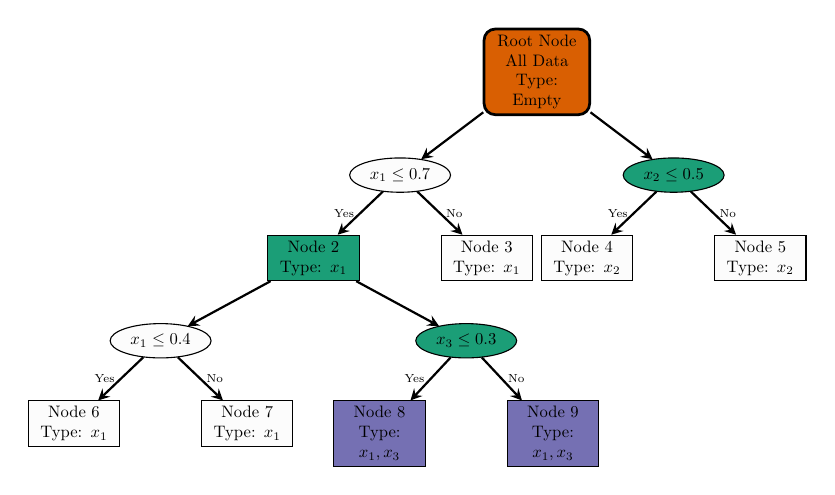
\begin{tikzpicture}[node distance=0.8cm and 1.1cm, scale=0.6, transform shape]

  % Root node
  \node (root) [root, text width=2cm, align=center] {Root Node\\All Data\\Type: Empty};

  % First level splits
  \node (b) [decision, below left=1cm and 1cm of root] {$x_1 \leq 0.7$};
  \node (e) [rpfuniquedecision, below right=1cm and 1cm of root] {$x_2 \leq 0.5$};

  % Connections from root
  \draw [arrow] (root) -- (b);
  \draw [arrow] (root) -- (e);

  % Nodes from first x1 split
  \node (c) [rpfunique, below left=1cm and 0.1cm of b, text width=1.7cm, align=center] {Node 2\\Type: $x_1$};
  \node (d) [internalnode, below right=1cm and 0.1cm of b, text width=1.7cm, align=center] {Node 3\\Type: $x_1$};

  % Connections from first split
  \draw [arrow] (b) -- node[label, left] {Yes} (c);
  \draw [arrow] (b) -- node[label, right] {No} (d);

  % Nodes from x2 split
  \node (f) [internalnode, below left=1cm and 0.1cm of e, text width=1.7cm, align=center] {Node 4\\Type: $x_2$};
  \node (g) [internalnode, below right=1cm and 0.1cm of e, text width=1.7cm, align=center] {Node 5\\Type: $x_2$};

  % Connections from x2 split
  \draw [arrow] (e) -- node[label, left] {Yes} (f);
  \draw [arrow] (e) -- node[label, right] {No} (g);

  % Further splits from Node 2
  \node (h) [decision, below left=1cm and 1.5cm of c] {$x_1 \leq 0.4$};
  \node (k) [rpfuniquedecision, below right=1cm and 1.5cm of c] {$x_3 \leq 0.3$};

  % Connections from Node 2
  \draw [arrow] (c) -- (h);
  \draw [arrow] (c) -- (k);

  % Nodes from x1 <= 0.4 split
  \node (i) [internalnode, below left=1cm and 0.1cm of h, text width=1.7cm, align=center] {Node 6\\Type: $x_1$};
  \node (j) [internalnode, below right=1cm and 0.1cm of h, text width=1.7cm, align=center] {Node 7\\Type: $x_1$};

  % Connections from x1 <= 0.4 split
  \draw [arrow] (h) -- node[label, left] {Yes} (i);
  \draw [arrow] (h) -- node[label, right] {No} (j);

  % Nodes from x3 split
  \node (l) [interaction, below left=1cm and 0.1cm of k, text width=1.7cm, align=center] {Node 8\\Type: $x_1,x_3$};
  \node (m) [interaction, below right=1cm and 0.1cm of k, text width=1.7cm, align=center] {Node 9\\Type: $x_1,x_3$};

  % Connections from x3 split
  \draw [arrow] (k) -- node[label, left] {Yes} (l);
  \draw [arrow] (k) -- node[label, right] {No} (m);

  % Further splits from Node 8
  % \node (n) [rpfuniquedecision, below=of l] {$x_3 \leq 0.2$};

  % % Connection from Node 8
  % \draw [arrow] (l) -- (n);

  % % Nodes from second x3 split
  % \node (o) [interaction, below left=1cm and 0.1cm of n, text width=1.7cm, align=center] {Node 10\\Type: $x_1,x_3$};
  % \node (p) [interaction, below right=1cm and 0.1cm of n, text width=1.7cm, align=center] {Node 11\\Type: $x_1,x_3$};

  % % Connections from second x3 split
  % \draw [arrow] (n) -- node[label, left] {Yes} (o);
  % \draw [arrow] (n) -- node[label, right] {No} (p);

  % Legend - moved to the right side, stacked vertically
  % \node (legend) [above right=0cm and 0.5cm of root, font=\bfseries, anchor=west] {Legend:};
  % \node (leg1) [root, below=0.2cm of legend, scale=0.8, text width=2cm, align=center, anchor=west] {Root Node};
  % \node (leg2) [decision, below=0.2cm of leg1, scale=0.8, text width=2cm, align=center, anchor=west] {CART-like Node};
  % \node (leg3) [rpfunique, below=0.2cm of leg2, scale=0.8, text width=2cm, align=center, anchor=west] {RPF-Unique Node};
  % \node (leg4) [interaction, below=0.2cm of leg3, scale=0.8, text width=2cm, align=center, anchor=west] {Interaction Node};

  % Key differences as numbered, well-positioned annotations
  % \node[font=\footnotesize, text width=2.4cm, red, align=left] at ($(root) + (1.5,-0.3)$) {1. Multiple splits from root};
  % \node[font=\footnotesize, text width=2.4cm, red, align=left] at ($(c) + (2.4,0)$) {2. Kept original leaf};
  % \node[font=\footnotesize, text width=2.4cm, red, align=left] at ($(l) + (1.6,0.3)$) {3. Interaction nodes};
  % \node[font=\footnotesize, text width=2.4cm, red, align=left] at ($(n) + (0,-1.5)$) {4. Only existing variables for split if max\_interaction=2};

\end{tikzpicture}
\end{document}
